\begin{frame}[t]{Example: How does a pattern predicate work?}
  \only<1-17>{sequence=}%
  \only<1-2>{\tt \textcolor{blue}{[13 2.0 6.0 4 "a" "an" "the" -5 2.0 3.0 4.0 7 8.0]}}%
  \only<3>{\tt [13 2.0 6.0 4 "a" "an" "the" -5 2.0 3.0 4.0 7 8.0]}%
  \only<4>{\tt [\colorbox{orange!30}{\Large 13} 2.0 6.0 4 "a" "an" "the" -5 2.0 3.0 4.0 7 8.0]}%
  \only<5>{\tt [13 \colorbox{orange!30}{\Large 2.0} 6.0 4 "a" "an" "the" -5 2.0 3.0 4.0 7 8.0]}%
  \only<6>{\tt [13 2.0 \colorbox{orange!30}{\Large 6.0} 4 "a" "an" "the" -5 2.0 3.0 4.0 7 8.0]}%
  \only<7>{\tt [13 2.0 6.0 \colorbox{orange!30}{\Large 4} "a" "an" "the" -5 2.0 3.0 4.0 7 8.0]}%
  \only<8>{\tt [13 2.0 6.0 4 \colorbox{orange!30}{\Large "a"} "an" "the" -5 2.0 3.0 4.0 7 8.0]}%
  \only<9>{\tt [13 2.0 6.0 4 "a" \colorbox{orange!30}{\Large "an"} "the" -5 2.0 3.0 4.0 7 8.0]}%
  \only<10>{\tt [13 2.0 6.0 4 "a" "an" \colorbox{orange!30}{\Large "the"} -5 2.0 3.0 4.0 7 8.0]}%
  \only<11>{\tt [13 2.0 6.0 4 "a" "an" "the" \colorbox{orange!30}{\Large -5} 2.0 3.0 4.0 7 8.0]}%
  \only<12>{\tt [13 2.0 6.0 4 "a" "an" "the" -5 \colorbox{orange!30}{\Large 2.0} 3.0 4.0 7 8.0]}%
  \only<13>{\tt [13 2.0 6.0 4 "a" "an" "the" -5 2.0 \colorbox{orange!30}{\Large 3.0} 4.0 7 8.0]}%
  \only<14>{\tt [13 2.0 6.0 4 "a" "an" "the" -5 2.0 3.0 \colorbox{orange!30}{\Large 4.0} 7 8.0]}%
  \only<15>{\tt [13 2.0 6.0 4 "a" "an" "the" -5 2.0 3.0 4.0 \colorbox{orange!30}{\Large 7} 8.0]}%
  \only<16>{\tt [13 2.0 6.0 4 "a" "an" "the" -5 2.0 3.0 4.0 7 \colorbox{orange!30}{\Large 8.0}]}%
  \only<17>{\tt [13 2.0 6.0 4 "a" "an" "the" -5 2.0 3.0 4.0 7 8.0]}%
 \only<18>{\textcolor{blue}{Decision procedure is $O(n)$,\Emph{independent of syntactical complexity} of the RTE.}}%

 \begin{columns}
   \begin{column}{0.4\textwidth}
     \only<2>{

       \bigskip

       Does the sequence match the pattern?
       \textcolor{greeny}{${(Int \cdot ( Double^{+} ~\vee String^{+}))^{+}}$}

       \bigskip

     
       We \textcolor{blue}{construct~a finite automaton} (DFA).
       
       \bigskip
       
       \Challenge{3} How to construct a finite automaton from an RTE? \Emph{Compile-time}}%
     \only<3,17,18>{\textcolor{greeny}{\LARGE $pattern={{(Int \cdot ( Double^{+} ~\vee String^{+}))^{+}}}$}\leavevmode\\[2cm]}%
     \only<4,7,11,15>{\textcolor{greeny}{\LARGE $pattern={{(\Emph{Int} \cdot ( Double^{+} ~\vee String^{+}))^{+}}}$}\leavevmode\\[2cm]}%
     \only<5,6,12-14,16>{\textcolor{greeny}{\LARGE $pattern={{(Int \cdot ( \Emph{Double}^{+} ~\vee String^{+}))^{+}}}$}\leavevmode\\[2cm]}%
     \only<8,9,10>{\textcolor{greeny}{\LARGE $pattern={{(Int \cdot ( Double^{+} ~\vee \Emph{String}^{+}))^{+}}}$}\leavevmode\\[2cm]}%
     \only<3-16>{\textcolor{orange}{\LARGE Does the sequence match the pattern?} \Emph{Run-time}}%
     \only<17>{\Emph{\LARGE Yes, it's a match!}}%
     \only<18>{
\includegraphics[height=3.cm]{exploding-head}}
   \end{column}
   \begin{column}{0.6\textwidth}
     \only<2,18>{\scalebox{0.95}{\documentclass{standalone}
  \usepackage{tikz}
  \usetikzlibrary{arrows.meta, automata, bending, positioning, shapes.misc}
  \tikzstyle{automaton}=[shorten >=1pt, >={Stealth[bend,round]}, initial text=]

\begin{document}
\begin{tikzpicture}[automaton, auto, thick]
  \node[state,initial,rounded rectangle] (0) {$0$};
  \node[state,rounded rectangle] (1) [right=20mm of 0] {$1$};
  \node[state,accepting,thick,rounded rectangle] (2) [above right=7mm and 30mm of 1] {$2$};
  \node[state,accepting,thick,rounded rectangle] (3) [below right=7mm and 30mm of 1] {$3$};
  \path[->] (0) edge node {$Int$} (1);
  \path[->] (1) edge[bend left=15]  node[pos=.8] {$Float$} (2);
  \path[->] (1) edge[bend right=15] node[swap] {$String$} (3);
  \path[->] (2) edge[bend left=15]  node {$Int$} (1);
  \path[->] (2) edge[loop above]    node {$Float$} (2);
  \path[->] (3) edge[bend right=15] node[swap] {$Int$} (1);
  \path[->] (3) edge[loop below]    node {$String$} (3);
\end{tikzpicture}
\end{document}
}}%
     \only<3>{\scalebox{0.95}{\documentclass{standalone}
  \usepackage{tikz}
  \usetikzlibrary{arrows.meta, automata, bending, positioning, shapes.misc}
  \tikzstyle{automaton}=[shorten >=1pt, >={Stealth[bend,round]}, initial text=]

\begin{document}
\begin{tikzpicture}[automaton, auto, thick]
  \node[state,initial,rounded rectangle,fill=yellow] (0) {$0$};
  \node[state,rounded rectangle] (1) [right=20mm of 0] {$1$};
  \node[state,accepting,thick,rounded rectangle] (2) [above right=7mm and 30mm of 1] {$2$};
  \node[state,accepting,thick,rounded rectangle] (3) [below right=7mm and 30mm of 1] {$3$};
  \path[->] (0) edge node {$Int$} (1);
  \path[->] (1) edge[bend left=15]  node[pos=.8] {$Float$} (2);
  \path[->] (1) edge[bend right=15] node[swap] {$String$} (3);
  \path[->] (2) edge[bend left=15]  node {$Int$} (1);
  \path[->] (2) edge[loop above]    node {$Float$} (2);
  \path[->] (3) edge[bend right=15] node[swap] {$Int$} (1);
  \path[->] (3) edge[loop below]    node {$String$} (3);
\end{tikzpicture}
\end{document}
}}%
     \only<4>{\scalebox{0.95}{\documentclass{standalone}
  \usepackage{tikz}
  \usetikzlibrary{arrows.meta, automata, bending, positioning, shapes.misc}
  \tikzstyle{automaton}=[shorten >=1pt, >={Stealth[bend,round]}, initial text=]

\begin{document}
\begin{tikzpicture}[automaton, auto, thick]
  \node[state,initial,rounded rectangle,fill=yellow] (0) {$0$};
  \node[state,rounded rectangle,fill=yellow] (1) [right=20mm of 0] {$1$};
  \node[state,accepting,thick,rounded rectangle] (2) [above right=7mm and 30mm of 1] {$2$};
  \node[state,accepting,thick,rounded rectangle] (3) [below right=7mm and 30mm of 1] {$3$};
  \path[->] (0) edge[orange, line width=3] node {$Int$} (1);
  \path[->] (1) edge[bend left=15]  node[pos=.8] {$Double$} (2);
  \path[->] (1) edge[bend right=15] node[swap] {$String$} (3);
  \path[->] (2) edge[bend left=15]  node {$Int$} (1);
  \path[->] (2) edge[loop above]    node {$Double$} (2);
  \path[->] (3) edge[bend right=15] node[swap] {$Int$} (1);
  \path[->] (3) edge[loop below]    node {$String$} (3);
\end{tikzpicture}
\end{document}
}}%
     \only<5>{\scalebox{0.95}{\documentclass{standalone}
  \usepackage{tikz}
  \usetikzlibrary{arrows.meta, automata, bending, positioning, shapes.misc}
  \tikzstyle{automaton}=[shorten >=1pt, >={Stealth[bend,round]}, initial text=]

\begin{document}
\begin{tikzpicture}[automaton, auto, thick]
  \node[state,initial,rounded rectangle] (0) {$0$};
  \node[state,rounded rectangle,fill=yellow] (1) [right=20mm of 0] {$1$};
  \node[state,accepting,thick,rounded rectangle,fill=yellow] (2) [above right=7mm and 30mm of 1] {$2$};
  \node[state,accepting,thick,rounded rectangle] (3) [below right=7mm and 30mm of 1] {$3$};
  \path[->] (0) edge node {$Int$} (1);
  \path[->] (1) edge[orange, line width=3pt, bend left=15]  node[pos=.8] {$Double$} (2);
  \path[->] (1) edge[bend right=15] node[swap] {$String$} (3);
  \path[->] (2) edge[bend left=15]  node {$Int$} (1);
  \path[->] (2) edge[loop above]    node {$Double$} (2);
  \path[->] (3) edge[bend right=15] node[swap] {$Int$} (1);
  \path[->] (3) edge[loop below]    node {$String$} (3);
\end{tikzpicture}
\end{document}
}}%
     \only<6>{\scalebox{0.95}{\documentclass{standalone}
  \usepackage{tikz}
  \usetikzlibrary{arrows.meta, automata, bending, positioning, shapes.misc}
  \tikzstyle{automaton}=[shorten >=1pt, >={Stealth[bend,round]}, initial text=]

\begin{document}
\begin{tikzpicture}[automaton, auto, thick]
  \node[state,initial,rounded rectangle] (0) {$0$};
  \node[state,rounded rectangle] (1) [right=20mm of 0] {$1$};
  \node[state,accepting,thick,rounded rectangle,fill=yellow] (2) [above right=7mm and 30mm of 1] {$2$};
  \node[state,accepting,thick,rounded rectangle] (3) [below right=7mm and 30mm of 1] {$3$};
  \path[->] (0) edge node {$Int$} (1);
  \path[->] (1) edge[bend left=15]  node[pos=.8] {$Double$} (2);
  \path[->] (1) edge[bend right=15] node[swap] {$String$} (3);
  \path[->] (2) edge[bend left=15]  node {$Int$} (1);
  \path[->] (2) edge[orange, line width=3pt, loop above]    node {$Double$} (2);
  \path[->] (3) edge[bend right=15] node[swap] {$Int$} (1);
  \path[->] (3) edge[loop below]    node {$String$} (3);
\end{tikzpicture}
\end{document}
}}%
     \only<7>{\scalebox{0.95}{\documentclass{standalone}
  \usepackage{tikz}
  \usetikzlibrary{arrows.meta, automata, bending, positioning, shapes.misc}
  \tikzstyle{automaton}=[shorten >=1pt, >={Stealth[bend,round]}, initial text=]

\begin{document}
\begin{tikzpicture}[automaton, auto, thick]
  \node[state,initial,rounded rectangle] (0) {$0$};
  \node[state,rounded rectangle,fill=yellow] (1) [right=20mm of 0] {$1$};
  \node[state,accepting,thick,rounded rectangle,fill=yellow] (2) [above right=7mm and 30mm of 1] {$2$};
  \node[state,accepting,thick,rounded rectangle] (3) [below right=7mm and 30mm of 1] {$3$};
  \path[->] (0) edge node {$Int$} (1);
  \path[->] (1) edge[bend left=15]  node[pos=.8] {$Double$} (2);
  \path[->] (1) edge[bend right=15] node[swap] {$String$} (3);
  \path[->] (2) edge[orange, line width=3pt, bend left=15]  node {$Int$} (1);
  \path[->] (2) edge[loop above]    node {$Double$} (2);
  \path[->] (3) edge[bend right=15] node[swap] {$Int$} (1);
  \path[->] (3) edge[loop below]    node {$String$} (3);
\end{tikzpicture}
\end{document}
}}%
     \only<8>{\scalebox{0.95}{\input{fig-3-1-String}}}%
     \only<9>{\scalebox{0.95}{\input{fig-3-3-String}}}%
     \only<10>{\scalebox{0.95}{\input{fig-3-3-String}}}%
     \only<11>{\scalebox{0.95}{\documentclass{standalone}
  \usepackage{tikz}
  \usetikzlibrary{arrows.meta, automata, bending, positioning, shapes.misc}
  \tikzstyle{automaton}=[shorten >=1pt, >={Stealth[bend,round]}, initial text=]

\begin{document}
\begin{tikzpicture}[automaton, auto, thick]
  \node[state,initial,rounded rectangle] (0) {$0$};
  \node[state,rounded rectangle,fill=yellow] (1) [right=20mm of 0] {$1$};
  \node[state,accepting,thick,rounded rectangle] (2) [above right=7mm and 30mm of 1] {$2$};
  \node[state,accepting,thick,rounded rectangle,fill=yellow] (3) [below right=7mm and 30mm of 1] {$3$};
  \path[->] (0) edge node {$Int$} (1);
  \path[->] (1) edge[bend left=15]  node[pos=.8] {$Double$} (2);
  \path[->] (1) edge[bend right=15] node[swap] {$String$} (3);
  \path[->] (2) edge[bend left=15]  node {$Int$} (1);
  \path[->] (2) edge[loop above]    node {$Double$} (2);
  \path[->] (3) edge[orange, line width=3pt, bend right=15] node[swap] {$Int$} (1);
  \path[->] (3) edge[loop below]    node {$String$} (3);
\end{tikzpicture}
\end{document}
}}%
     \only<12>{\scalebox{0.95}{\documentclass{standalone}
  \usepackage{tikz}
  \usetikzlibrary{arrows.meta, automata, bending, positioning, shapes.misc}
  \tikzstyle{automaton}=[shorten >=1pt, >={Stealth[bend,round]}, initial text=]

\begin{document}
\begin{tikzpicture}[automaton, auto, thick]
  \node[state,initial,rounded rectangle] (0) {$0$};
  \node[state,rounded rectangle,fill=yellow] (1) [right=20mm of 0] {$1$};
  \node[state,accepting,thick,rounded rectangle,fill=yellow] (2) [above right=7mm and 30mm of 1] {$2$};
  \node[state,accepting,thick,rounded rectangle] (3) [below right=7mm and 30mm of 1] {$3$};
  \path[->] (0) edge node {$Int$} (1);
  \path[->] (1) edge[orange, line width=3pt, bend left=15]  node[pos=.8] {$Double$} (2);
  \path[->] (1) edge[bend right=15] node[swap] {$String$} (3);
  \path[->] (2) edge[bend left=15]  node {$Int$} (1);
  \path[->] (2) edge[loop above]    node {$Double$} (2);
  \path[->] (3) edge[bend right=15] node[swap] {$Int$} (1);
  \path[->] (3) edge[loop below]    node {$String$} (3);
\end{tikzpicture}
\end{document}
}}%
     \only<13>{\scalebox{0.95}{\documentclass{standalone}
  \usepackage{tikz}
  \usetikzlibrary{arrows.meta, automata, bending, positioning, shapes.misc}
  \tikzstyle{automaton}=[shorten >=1pt, >={Stealth[bend,round]}, initial text=]

\begin{document}
\begin{tikzpicture}[automaton, auto, thick]
  \node[state,initial,rounded rectangle] (0) {$0$};
  \node[state,rounded rectangle] (1) [right=20mm of 0] {$1$};
  \node[state,accepting,thick,rounded rectangle,fill=yellow] (2) [above right=7mm and 30mm of 1] {$2$};
  \node[state,accepting,thick,rounded rectangle] (3) [below right=7mm and 30mm of 1] {$3$};
  \path[->] (0) edge node {$Int$} (1);
  \path[->] (1) edge[bend left=15]  node[pos=.8] {$Double$} (2);
  \path[->] (1) edge[bend right=15] node[swap] {$String$} (3);
  \path[->] (2) edge[bend left=15]  node {$Int$} (1);
  \path[->] (2) edge[orange, line width=3pt, loop above]    node {$Double$} (2);
  \path[->] (3) edge[bend right=15] node[swap] {$Int$} (1);
  \path[->] (3) edge[loop below]    node {$String$} (3);
\end{tikzpicture}
\end{document}
}}%
     \only<14>{\scalebox{0.95}{\documentclass{standalone}
  \usepackage{tikz}
  \usetikzlibrary{arrows.meta, automata, bending, positioning, shapes.misc}
  \tikzstyle{automaton}=[shorten >=1pt, >={Stealth[bend,round]}, initial text=]

\begin{document}
\begin{tikzpicture}[automaton, auto, thick]
  \node[state,initial,rounded rectangle] (0) {$0$};
  \node[state,rounded rectangle] (1) [right=20mm of 0] {$1$};
  \node[state,accepting,thick,rounded rectangle,fill=yellow] (2) [above right=7mm and 30mm of 1] {$2$};
  \node[state,accepting,thick,rounded rectangle] (3) [below right=7mm and 30mm of 1] {$3$};
  \path[->] (0) edge node {$Int$} (1);
  \path[->] (1) edge[bend left=15]  node[pos=.8] {$Double$} (2);
  \path[->] (1) edge[bend right=15] node[swap] {$String$} (3);
  \path[->] (2) edge[bend left=15]  node {$Int$} (1);
  \path[->] (2) edge[orange, line width=3pt, loop above]    node {$Double$} (2);
  \path[->] (3) edge[bend right=15] node[swap] {$Int$} (1);
  \path[->] (3) edge[loop below]    node {$String$} (3);
\end{tikzpicture}
\end{document}
}}%
     \only<15>{\scalebox{0.95}{\documentclass{standalone}
  \usepackage{tikz}
  \usetikzlibrary{arrows.meta, automata, bending, positioning, shapes.misc}
  \tikzstyle{automaton}=[shorten >=1pt, >={Stealth[bend,round]}, initial text=]

\begin{document}
\begin{tikzpicture}[automaton, auto, thick]
  \node[state,initial,rounded rectangle] (0) {$0$};
  \node[state,rounded rectangle,fill=yellow] (1) [right=20mm of 0] {$1$};
  \node[state,accepting,thick,rounded rectangle,fill=yellow] (2) [above right=7mm and 30mm of 1] {$2$};
  \node[state,accepting,thick,rounded rectangle] (3) [below right=7mm and 30mm of 1] {$3$};
  \path[->] (0) edge node {$Int$} (1);
  \path[->] (1) edge[bend left=15]  node[pos=.8] {$Double$} (2);
  \path[->] (1) edge[bend right=15] node[swap] {$String$} (3);
  \path[->] (2) edge[orange, line width=3pt, bend left=15]  node {$Int$} (1);
  \path[->] (2) edge[loop above]    node {$Double$} (2);
  \path[->] (3) edge[bend right=15] node[swap] {$Int$} (1);
  \path[->] (3) edge[loop below]    node {$String$} (3);
\end{tikzpicture}
\end{document}
}}%
     \only<16>{\scalebox{0.95}{\documentclass{standalone}
  \usepackage{tikz}
  \usetikzlibrary{arrows.meta, automata, bending, positioning, shapes.misc}
  \tikzstyle{automaton}=[shorten >=1pt, >={Stealth[bend,round]}, initial text=]

\begin{document}
\begin{tikzpicture}[automaton, auto, thick]
  \node[state,initial,rounded rectangle] (0) {$0$};
  \node[state,rounded rectangle,fill=yellow] (1) [right=20mm of 0] {$1$};
  \node[state,accepting,thick,rounded rectangle,fill=yellow] (2) [above right=7mm and 30mm of 1] {$2$};
  \node[state,accepting,thick,rounded rectangle] (3) [below right=7mm and 30mm of 1] {$3$};
  \path[->] (0) edge node {$Int$} (1);
  \path[->] (1) edge[orange, line width=3pt, bend left=15]  node[pos=.8] {$Double$} (2);
  \path[->] (1) edge[bend right=15] node[swap] {$String$} (3);
  \path[->] (2) edge[bend left=15]  node {$Int$} (1);
  \path[->] (2) edge[loop above]    node {$Double$} (2);
  \path[->] (3) edge[bend right=15] node[swap] {$Int$} (1);
  \path[->] (3) edge[loop below]    node {$String$} (3);
\end{tikzpicture}
\end{document}
}}%
     \only<17>{\scalebox{0.95}{\documentclass{standalone}
  \usepackage{tikz}
  \usetikzlibrary{arrows.meta, automata, bending, positioning, shapes.misc}
  \tikzstyle{automaton}=[shorten >=1pt, >={Stealth[bend,round]}, initial text=]

\begin{document}
\begin{tikzpicture}[automaton, auto, thick]
  \node[state,initial,rounded rectangle] (0) {$0$};
  \node[state,rounded rectangle] (1) [right=20mm of 0] {$1$};
  \node[state,accepting,thick,rounded rectangle,fill=greeny] (2) [above right=7mm and 30mm of 1] {$2$};
  \node[state,accepting,thick,rounded rectangle] (3) [below right=7mm and 30mm of 1] {$3$};
  \path[->] (0) edge node {$Int$} (1);
  \path[->] (1) edge[bend left=15]  node[pos=.8] {$Float$} (2);
  \path[->] (1) edge[bend right=15] node[swap] {$String$} (3);
  \path[->] (2) edge[bend left=15]  node {$Int$} (1);
  \path[->] (2) edge[loop above]    node {$Float$} (2);
  \path[->] (3) edge[bend right=15] node[swap] {$Int$} (1);
  \path[->] (3) edge[loop below]    node {$String$} (3);
\end{tikzpicture}
\end{document}
}}%
   \end{column}
 \end{columns}
\end{frame}



\begin{frame}{Deterministic (DFA) vs Non-deterministic (NFA)}

  %% \only<1>{1}%
  %% \only<2>{2}%
  %% \only<3>{3}%
  %% \only<4>{4}%
  %% \only<5>{5}%
  %% \only<6>{6}%
  %% \only<7>{7}%
  %% \only<8>{8}%
  %% \only<9>{9}%
  %% \only<10>{10}%
  \only<1,9>{Suppose sequence = \code{[2,  3, 5.6F]}}%
  %\only<10>{Suppose sequence = \code{[2,  3, 5.6F]}}%
  \only<2,4,6,7>{Suppose sequence = \code{[2,  \colorbox{orange!30}{\Large 3}, 5.6F]}}%
  \only<3,5,8>{Suppose sequence = \code{[2,  3, \colorbox{orange!30}{\Large 5.6F}]}}%

  \begin{columns}[T]
    \begin{column}{0.3\textwidth}
      \centering
      
      \only<1-9>{\begin{align*}
        Int&\subseteq Number\\
        Int &\cap Number \neq \emptyset
      \end{align*}%
      \scalebox{0.8}{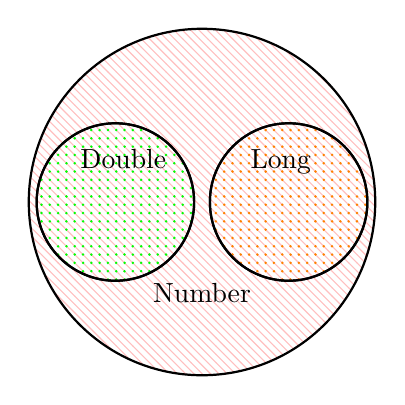
\begin{tikzpicture}[thick]
\usetikzlibrary{patterns}
  
\draw[pattern=north west lines, pattern color=pink] (0,0) circle (2.2);
\draw[pattern=dots, pattern color=orange
] (1.1,0) circle (1.0);
\draw[pattern=dots, pattern color=green
] (-1.1,0) circle (1.0);
\draw (1,0.8)     node [text=black,below] {Long};
\draw (-1,0.8)     node [text=black,below] {Double};
\draw (1.1,0) circle (1)  ;
\draw (-1.1,0) circle (1)  ;
\draw (0.0,-0.9) node [text=black,below] {Number};
\end{tikzpicture}

}}%
      %% \only<11>{\begin{align*}
      %%   Int&\subseteq Int\\
      %%   Int &\cap String = \emptyset
      %%   \end{align*}
      %%   \scalebox{1}{\begin{tikzpicture}[thick]
\usetikzlibrary{patterns}
  
\draw[pattern=dots, pattern color=orange
] (0.1,0) circle (1.5);
\draw[pattern=north east lines, pattern color=gold
] (0.1,0) circle (0.6);

\draw (0,0.3)     node [text=black,below] {Odd};
\draw (0,1.2)     node [text=black,below] {Int};
\end{tikzpicture}

}}
    \end{column}%
    \begin{column}{0.7\textwidth}
      \only<1>{\scalebox{0.95}{\documentclass{standalone}
  \usepackage{tikz}
  \usetikzlibrary{arrows.meta, automata, bending, positioning, shapes.misc}
  \tikzstyle{automaton}=[shorten >=1pt, >={Stealth[bend,round]}, initial text=]

\begin{document}
\begin{tikzpicture}[automaton, auto, thick]
  \node[state,initial,rounded rectangle] (0) {$0$};
  \node[state,rounded rectangle] (1) [right=10mm of 0] {$1$};
  \node[state,rounded rectangle] (2) [above right=7mm and 20mm of 1] {$2$};
  \node[state,accepting] (3) [right=20mm of 2] {$3$};
  \node[state,rounded rectangle] (4) [below right=7mm and 20mm of 1] {$4$};
  \node[state,accepting] (5) [right=20mm of 4] {$5$};
  \path[->] (0) edge node {$Long$} (1);
  \path[->] (1) edge[color=nondeterministic, line width=3pt, bend left=15]  node[pos=.8] {$Long$} (2);
  \path[->] (2) edge  node {$String$} (3);
  \path[->] (1) edge[color=nondeterministic, line width=3pt, bend right=15] node[swap] {$Number$} (4);
  \path[->] (4) edge  node {$Double$} (5);
\end{tikzpicture}
\end{document}
}}%
      \only<2>{\scalebox{0.95}{\documentclass{standalone}
  \usepackage{tikz}
  \usetikzlibrary{arrows.meta, automata, bending, positioning, shapes.misc}
  \tikzstyle{automaton}=[shorten >=1pt, >={Stealth[bend,round]}, initial text=]

\begin{document}
\begin{tikzpicture}[automaton, auto, thick]
  \node[state,initial,rounded rectangle] (0) {$0$};
  \node[state,rounded rectangle] (1) [fill=yellow,right=10mm of 0] {$1$};
  \node[state,rounded rectangle] (2) [fill=yellow,above right=7mm and 20mm of 1] {$2$};
  \node[state,accepting] (3) [right=20mm of 2] {$3$};
  \node[state,rounded rectangle] (4) [below right=7mm and 20mm of 1] {$4$};
  \node[state,accepting] (5) [right=20mm of 4] {$5$};
  \path[->] (0) edge node {$Long$} (1);
  \path[->] (1) edge[color=orange, line width=3pt, bend left=15]  node[pos=.8] {$Long$} (2);
  \path[->] (2) edge  node {$String$} (3);
  \path[->] (1) edge[bend right=15] node[swap] {$Number$} (4);
  \path[->] (4) edge  node {$Double$} (5);
\end{tikzpicture}
\end{document}
}}%
      \only<3>{\scalebox{0.95}{\documentclass{standalone}
  \usepackage{tikz}
  \usetikzlibrary{arrows.meta, automata, bending, positioning, shapes.misc}
  \tikzstyle{automaton}=[shorten >=1pt, >={Stealth[bend,round]}, initial text=]

\begin{document}
\begin{tikzpicture}[automaton, auto, thick]
  \node[state,initial,rounded rectangle] (0) {$0$};
  \node[state,rounded rectangle] (1) [right=10mm of 0] {$1$};
  \node[state,rounded rectangle] (2) [fill=yellow,above right=7mm and 20mm of 1] {$2$};
  \node[state,accepting] (3) [fill=yellow, right=20mm of 2] {$3$};
  \node[state,rounded rectangle] (4) [below right=7mm and 20mm of 1] {$4$};
  \node[state,accepting] (5) [right=20mm of 4] {$5$};
  \path[->] (0) edge node {$Int$} (1);
  \path[->] (1) edge[bend left=15]  node[pos=.8] {$Int$} (2);
  \path[->] (2) edge[dashed, line width=3pt, color=red]  node {$\cancel{String}$} (3);
  \path[->] (1) edge[bend right=15] node[swap] {$Number$} (4);
  \path[->] (4) edge  node {$Float$} (5);
\end{tikzpicture}
\end{document}
}}%
      \only<4>{\scalebox{0.95}{\documentclass{standalone}
  \usepackage{tikz}
  \usetikzlibrary{arrows.meta, automata, bending, positioning, shapes.misc}
  \tikzstyle{automaton}=[shorten >=1pt, >={Stealth[bend,round]}, initial text=]

\begin{document}
\begin{tikzpicture}[automaton, auto, thick]
  \node[state,initial,rounded rectangle] (0) {$0$};
  \node[state,rounded rectangle] (1) [fill=yellow,right=10mm of 0] {$1$};
  \node[state,rounded rectangle] (2) [above right=7mm and 20mm of 1] {$2$};
  \node[state,accepting] (3) [right=20mm of 2] {$3$};
  \node[state,rounded rectangle] (4) [fill=yellow, below right=7mm and 20mm of 1] {$4$};
  \node[state,accepting] (5) [right=20mm of 4] {$5$};
  \path[->] (0) edge node {$Int$} (1);
  \path[->] (1) edge[bend left=15]  node[pos=.8] {$Int$} (2);
  \path[->] (2) edge  node {$String$} (3);
  \path[->] (1) edge[color=orange, line width=3pt, bend right=15] node[swap] {$Number$} (4);
  \path[->] (4) edge  node {$Float$} (5);
\end{tikzpicture}
\end{document}
}}%
      \only<5>{\scalebox{0.95}{\documentclass{standalone}
  \usepackage{tikz}
  \usetikzlibrary{arrows.meta, automata, bending, positioning, shapes.misc}
  \tikzstyle{automaton}=[shorten >=1pt, >={Stealth[bend,round]}, initial text=]

\begin{document}
\begin{tikzpicture}[automaton, auto, thick]
  \node[state,initial,rounded rectangle] (0) {$0$};
  \node[state,rounded rectangle] (1) [right=10mm of 0] {$1$};
  \node[state,rounded rectangle] (2) [above right=7mm and 20mm of 1] {$2$};
  \node[state,accepting] (3) [right=20mm of 2] {$3$};
  \node[state,rounded rectangle] (4) [fill=yellow, below right=7mm and 20mm of 1] {$4$};
  \node[state,accepting] (5) [fill=yellow,right=20mm of 4] {$5$};
  \path[->] (0) edge node {$Int$} (1);
  \path[->] (1) edge[bend left=15]  node[pos=.8] {$Int$} (2);
  \path[->] (2) edge  node {$String$} (3);
  \path[->] (1) edge[bend right=15] node[swap] {$Number$} (4);
  \path[->] (4) edge[color=orange, line width=3pt]  node {$Float$} (5);
\end{tikzpicture}
\end{document}
}}%
      
      \only<4,5>{
\includegraphics[height=1.5cm]{red-head}\LARGE Backtracking $\implies O(2^n)$}%
      \only<6>{\scalebox{0.95}{\documentclass{standalone}
  \usepackage{tikz}
  \usetikzlibrary{arrows.meta, automata, bending, positioning, shapes.misc}
  \tikzstyle{automaton}=[shorten >=1pt, >={Stealth[bend,round]}, initial text=]

\begin{document}
\begin{tikzpicture}[automaton, auto, thick]
  \node[state,initial,rounded rectangle] (0) {$0$};
  \node[state,rounded rectangle] (1) [right=10mm of 0] {$1$};
  \node[state,rounded rectangle] (2) [above right=7mm and 20mm of 1] {$2$};
  \node[state,accepting] (3) [right=40mm of 1] {$3$};
  \node[state,rounded rectangle] (4) [below right=7mm and 20mm of 1] {$4$};
  \path[->] (0) edge node {$Int$} (1);
  \path[->] (1) edge[color=deterministic, line width=3pt, bend left=15]  node[pos=.8] {$Int$} (2);
  \path[->] (2) edge  node {$Float\cup String$} (3);
  \path[->] (1) edge[color=deterministic, line width=3pt, bend right=15] node[swap] {$Number \cap \overline{Int}$} (4);
  \path[->] (4) edge  node {$Float$} (3);
\end{tikzpicture}
\end{document}
}\\
      Deterministic Choice between $Int$ vs $Number\cap\overline{Int}$}%2
      \only<7>{\scalebox{0.95}{\documentclass{standalone}
  \usepackage{tikz}
  \usetikzlibrary{arrows.meta, automata, bending, positioning, shapes.misc}
  \tikzstyle{automaton}=[shorten >=1pt, >={Stealth[bend,round]}, initial text=]

\begin{document}
\begin{tikzpicture}[automaton, auto, thick]
  \node[state,initial,rounded rectangle] (0) {$0$};
  \node[state,rounded rectangle] (1) [fill=yellow, right=10mm of 0] {$1$};
  \node[state,rounded rectangle] (2) [fill=yellow, above right=7mm and 20mm of 1] {$2$};
  \node[state,accepting] (3) [right=40mm of 1] {$3$};
  \node[state,rounded rectangle] (4) [below right=7mm and 20mm of 1] {$4$};
  \path[->] (0) edge node {$Long$} (1);
  \path[->] (1) edge[color=orange, line width=3pt, bend left=15]  node[pos=.8] {$Long$} (2);
  \path[->] (2) edge  node {$Double\cup String$} (3);
  \path[->] (1) edge[bend right=15] node[swap] {$Number \cap \overline{Long}$} (4);
  \path[->] (4) edge  node {$Double$} (3);
\end{tikzpicture}
\end{document}
}}%
      \only<8>{\scalebox{0.95}{\documentclass{standalone}
  \usepackage{tikz}
  \usetikzlibrary{arrows.meta, automata, bending, positioning, shapes.misc}
  \tikzstyle{automaton}=[shorten >=1pt, >={Stealth[bend,round]}, initial text=]

\begin{document}
\begin{tikzpicture}[automaton, auto, thick]
  \node[state,initial,rounded rectangle] (0) {$0$};
  \node[state,rounded rectangle] (1) [right=10mm of 0] {$1$};
  \node[state,rounded rectangle] (2) [fill=yellow,above right=7mm and 20mm of 1] {$2$};
  \node[state,accepting] (3) [fill=yellow, right=40mm of 1] {$3$};
  \node[state,rounded rectangle] (4) [below right=7mm and 20mm of 1] {$4$};
  \path[->] (0) edge node {$Long$} (1);
  \path[->] (1) edge[bend left=15]  node[pos=.8] {$Long$} (2);
  \path[->] (1) edge[bend right=15] node[swap] {$Number \cap \overline{Long}$} (4);
  \path[->] (4) edge  node {$Double$} (3);
  \path[->] (2) edge[color=orange, line width=3pt]  node {$Double\cup String$} (3);
\end{tikzpicture}
\end{document}
}}%
      \only<9>{\scalebox{0.8}{\documentclass{standalone}
  \usepackage{tikz}
  \usetikzlibrary{arrows.meta, automata, bending, positioning, shapes.misc}
  \tikzstyle{automaton}=[shorten >=1pt, >={Stealth[bend,round]}, initial text=]

\begin{document}
\begin{tikzpicture}[automaton, auto, thick]
  \node[state,initial,rounded rectangle] (0) {$0$};
  \node[state,rounded rectangle] (1) [right=10mm of 0] {$1$};
  \node[state,rounded rectangle] (2) [above right=7mm and 20mm of 1] {$2$};
  \node[state,accepting] (3) [right=40mm of 1] {$3$};
  \node[state,rounded rectangle] (4) [below right=7mm and 20mm of 1] {$4$};
  \path[->] (0) edge node {$Int$} (1);
  \path[->] (1) edge[color=deterministic, line width=3pt, bend left=15]  node[pos=.8] {$Int$} (2);
  \path[->] (2) edge  node {$Float\cup String$} (3);
  \path[->] (1) edge[color=deterministic, line width=3pt, bend right=15] node[swap] {$Number \cap \overline{Int}$} (4);
  \path[->] (4) edge  node {$Float$} (3);
\end{tikzpicture}
\end{document}
}}%
      %\only<10>{\scalebox{0.8}{\documentclass{standalone}
  \usepackage{tikz}
  \usetikzlibrary{arrows.meta, automata, bending, positioning, shapes.misc}
  \tikzstyle{automaton}=[shorten >=1pt, >={Stealth[bend,round]}, initial text=]

\begin{document}
\begin{tikzpicture}[automaton, auto, thick]
  \node[state,initial,rounded rectangle] (0) {$0$};
  \node[state,rounded rectangle] (1) [right=10mm of 0] {$1$};
  \node[state,rounded rectangle] (2) [above right=7mm and 20mm of 1] {$2$};
  \node[state,accepting] (3) [right=40mm of 1] {$3$};
  \node[state,rounded rectangle] (4) [below right=7mm and 20mm of 1] {$4$};
  \path[->] (0) edge node {$Int$} (1);
  \path[->] (1) edge[color=deterministic, line width=3pt, bend left=15]  node[pos=.8] {$Int$} (2);
  \path[->] (2) edge  node {$Float\cup String$} (3);
  \path[->] (1) edge[color=deterministic, line width=3pt, bend right=15] node[swap] {$Number \cap \overline{Int}$} (4);
  \path[->] (4) edge  node {$Float$} (3);
\end{tikzpicture}
\end{document}
}}%
      %\only<11>{\scalebox{0.8}{\documentclass{standalone}
  \usepackage{tikz}
  \usetikzlibrary{arrows.meta, automata, bending, positioning, shapes.misc}
  \tikzstyle{automaton}=[shorten >=1pt, >={Stealth[bend,round]}, initial text=]

\begin{document}
\begin{tikzpicture}[automaton, auto, thick]
  \node[state,initial,rounded rectangle] (0) {$0$};
  \node[state,rounded rectangle] (1) [right=10mm of 0] {$1$};
  \node[state,rounded rectangle] (2) [above right=7mm and 20mm of 1] {$2$};
  \node[state,accepting] (3) [right=40mm of 1] {$3$};
  \node[state,rounded rectangle] (4) [below right=7mm and 20mm of 1] {$4$};
  \path[->] (0) edge node {$Long$} (1);
  \path[->] (1) edge[color=deterministic, line width=3pt, bend left=15]  node[pos=.8] {$String \cup (Long \cap Odd)$} (2);
  \path[->] (2) edge  node {$Double\cup String$} (3);
  \path[->] (1) edge[color=indeterminate,style=dashed,line width=3pt, bend right=15] node[swap] {$Long \cap \overline{Odd}$} (4);
  \path[->] (4) edge  node {$Double$} (3);
\end{tikzpicture}
\end{document}
}}%
      \only<9->{}
      \only<9>{\Challenge{4} How to partition types? \\
        \Eg, type decomposition\\\quad\textcolor{greeny}{$\{String,Int,Number\}\to\{String,Int,Number\cap\overline{Int}\}$}}%
      %\only<10>{\Challenge{5} How to optimize run-time type checks?}%
      %\only<11>{\Challenge{6} How to check habitation?\\In spite of \emph{indeterminate} transitions.}%
    \end{column}
  \end{columns}
\end{frame}
